\chapter{Fundamentação Teórica}
\addcontentsline{toc}{chapter}{Fundamentação Teórica}

Aprendizado de máquina é uma disciplina focada em duas questões \
interelacionadas: Como construir sistemas que automaticamente melhoram \
por meio da experiência? e quais as leis estatisticas, \
computacionais e da teoria da informação que governam todos os sistemas \
de aprendizagem, incluindo computadores, seres humanos, e organizações?.
O estudo de aprendizado de máquina é importante tanto para responder a essas \
questões fundamentais de Engenharia e Ciência, quanto pelas aplicações \
computacionais que tem produzido \cite{Jordan}.

Um problema de aprendizado, pode ser colocado como um problema que reside em \
melhorar uma medida de performance, quando se executa alguma tarefa, \
através de algum tipo de experiência de treinamento \cite{Jordan}.

% Talvez mover esse bloco pra introdução
Para viabilizar o aprendizado de máquina, é necessário primeiramente \
entender os dados que serão utilizados no processo de aprendizado. \
Para entender esses dados lançaremos mão de técnicas e conceitos \
estatísticos, que nos permitirão construir um modelo probabilístico \
que represente, por meio de uma função $f$, \
variáveis de entrada e de saída que compõe os dados com que estamos lidando. \
O fato de estarmos lidando com uma entrada e uma saída conhecida faz com \
que nosso estudo se enquadre no \textit{aprendizado supervisionado}. \
Por outro lado, se no contexto do aprendizado, \
apenas dados de entrada estão disponíveis, \
é possível partir para o \textit{aprendizado não supervisionado}.

Para o aprendizado supervionado, o conjunto de dados utilizado \
no treinamento será formado pelos dados em si, e pela saída esperada \
para esses dados\cite{Louridas}. \
Segundo \cite{James}, aprendizado estatístico supervisionado envolve \
construir um modelo estatístico para prever ou estimar, \
uma saída a partir de uma ou mais entradas.


% Falar do alinhamento entre estatística e ciência da computação.

A disciplina de aprendizado de máquina pode ser subdividida da seguinte forma:
% TODO: Essa imagem tá muito pequena, aumentar a resolução.
\begin{figure}[h]
	\centering
	\label{fig01}
        \includegraphics[scale=0.48]{figuras/mind1.eps}
	\caption{Abordagens para aprendizado de máquina}
\end{figure}
Neste capitulo iremos direcionar nossos estudos para \
o aprendizado supervisionado, pois ele é a base para o estudo de inferência.

\section{Aprendizado Estatístico}

Modelos probabilísticos, que representam uma distribuição probabilistica \
sobre variáveis randomicas, provê um conjuto de ferramentas sólidas \
e com princípios para que problemas de incerteza \
possam ser resolvidos\cite{Sun}. \
Modelos probabilísticos podem ser lineares e não lineares.

Modelos probabilisticos lineares descrevem uma variável dependente contínua, \
como uma função de uma ou mais variáveis independentes, \
possibilitando relacionar cada entrada à saída esperada. \
Podemos definir então, que a entrada do nosso modelo probabilístico será um \
conjunto de dados representados aqui pelo simbolo $X$, \
e a nossa saída sendo representada pelo simbolo $Y$.  \
$X$ pode ser chamada de diversas formas, como preditor, \
variáveis independentes, características ou simplesmente variáveis.
O simbolo Y é normalmente chamado de resposta, ou variável dependente. \

Se consideramos um segundo exemplo dado por \cite{James}, em que o salário \
de um indivíduo é deduzido a partir de fatores como a sua idade, \
escolaridade e o ano em que os dados foram coletados. \
Temos que $X = \{idade, escolaridade, ano\}$, enquanto Y representa \
o salário, ou seja, o fator que varia, conforme $X_1(idade)$,
$X_2(escolaridade)$ e $X_3(ano)$ variam.\
Poderiamos ter $p$ variáveis para $X$, nesse caso $p$ é igual a 3. \
Podemos estabelecer também, que para cada $X_p$, \
teremos uma amostra de tamanho $n$. No exemplo dado por \cite{James}, \
poderíamos ter uma amostra de tamanho $n$(vários valores de salário) \
para a váriável independente $X_1$.
Essa relação entre $p$ e $n$ nos permite estruturar \
esses dados matricialmente, \
aonde $X$ pode ser escrito como $p$x$n$\cite{James}.

$X$ pode ser definida como

\[
X_{i,j} = \begin{matrix}
x_{1,1} & x_{1,2} & \cdots & x_{1,j} \\
x_{2,1} & x_{2,2} & \cdots & x_{2,j} \\
\vdots  & \vdots  & \ddots & \vdots  \\
x_{i,1} & x_{i,2} & \cdots & x_{i,j} \\
\end{matrix}
\]

Sendo que cada coluna representa $p$ e cada linha \
representa $n$. Nesse contexto $x_i$ é um vetor de tamanho $p$, \
em que cada elemento do mesmo representa um valor de $n$ atribuído \
a variável $p$ de posição $x_i$.

\[
X_{i} = \begin{matrix}
x_{i,1} \\
x_{i,2} \\
\vdots  \\
x_{i,3} \\
\end{matrix}
\]

Da  forma $x_j$ é um vetor de tamanho $n$, em que cada \
elemento representa uma valor da amostra de $n$ para uma \
variável $p$ específica.

\[
X_{j} = \begin{matrix}
x_{j,1} \\
x_{j,2} \\
\vdots  \\
x_{j,3} \\
\end{matrix}
\]

Podemos então representar essa relação entre $X$ e $Y$ da seguinte forma:

\[
  Y = f(X) + e
\]

$f$ é uma função fixa mas desconhecida de $X_1...X_p$, \
e $e$ é o termo de erro randomico, que é independente de $X$ \
e tem media zero. Essa formulação pode ser dita como ideal e teórica, \
uma vez que a função $f$ utilizada na prática, e o valor $Y$ encontrado \
como resultado, são estimativas, construidas a partir do \
aprendizado estatístico.
Podemos afirmar que $f$ representa a informação \textit{sistematica} \
que $X$ provê em releação a $Y$\cite{Jordan}.
Para definirmos $f$ devemos primeiro compreender a diferença \
entre inferência e predição.

\subsection{Predição}
Quando o objetivo do aprendizado reside em deduzir ou \
estimar um valor de $Y$, dado $X$, temos uma situação de predição. \
Podemos realizar essa predição utilizando
\[
  Y^* = f^*(X)
\]

$f^*$ é a estimativa para $f$, $Y^*$ é o valor previsto para $Y$. \
A precisão de $Y^*$ como uma previsão de $Y$ depende de dois valores, \
chamados de \textit{erro reduzivel} e \textit{erro irreduzivel}. \
No geral, $f^*$ não será uma estimativa perfeita de $f$, \
e essa imperfeição irá naturalmente, adicionar \
erros no resultado\cite{Jordan}.  O \textit{erro reduzivel} está \
relacionado ao erro de precisão de $f$. Ele é chamado de reduzível \
justamente pelo fato de que, por meio do treinamento, \
a precisão de $f^*$ pode ser cada vez melhor. Se uma amostra $n$ \
muito grande está disponível($n$ tende ao infinito) $f^*$ \
irá convergir para $f$\cite{Malhotra}.
O erro \textit{erro irreduzivel} está relacionado ao erro $e$. \
Neste caso o erro independe de $X$, ou seja, não importa quão bom \
seja a nossa amostra de dados, muito menos o quão apropriada é a \
técnica de aprendizado estatístico utilizado, sempre haverá um \
erro $e$ que influência a precisão das previsões\cite{Jordan}.

A teoria de aprendizado estatístico tem por objetivo dar as \
condições necessárias e suficientes no que tange aos modelos \
estatísticos, que irá garantir a consistência da estimativa de $f^*$, \
o que implica na convergência para $f$\cite{Malhotra}.

Aplicando a predição ao exemplo dado anteriormente do salário, \
poderíamos, estimando a função $f$, deduzir o salário de um indivíduo \
a partir das variáveis de idade, escolaridade e ano de coleta dos dados. \
Abordagens não lineares são comumente utilizadas para estimar $f$, \
quando se tem uma situação de predição.

\subsubsection{classificação}

Uma tarefa pode ser entendida como o processo de categorizar um dado, \
que será utilizado como entrada do algorítmo de aprendizado de \
máquina escolhido. Um bom exemplo dado por \cite{Jordan}, \
é a classificação de uma transação bancária como fraudulenta ou não. \
A tarefa reside exatamente na categorização. O quão precisa essa \
categorização é, depende da forma como o algorítmo escolhido para \
atender tal demanda é treinado. A maneira como esses dados \
são categorizados varia de acordo com o algorítmo selecionado para \
a classificação. Cada algorítmo espera que esses dados sejam \
modelados de uma forma ou de outra, assunto que será \
abordado ao longo deste capítulo.

\subsubsection{regressão}

%TODO: Falar sobre regressão

\subsection{Inferência}

Quando o objetivo do aprendizado é entender como o conjunto de \
variáveis independentes $X$, influênciam a variável dependente $Y$, temos \
uma situação de inferência. Da mesma forma que no processo de predição, \
temos a tarefa de estimar $f$, mas o objetivo final do aprendizado \
não é deduzir um valor para $Y$, e sim entender como $Y$ muda em função de $X_1...X_p$.

Nesse contexto, é necessário responder a algumas questões:

\begin{itemize}
\item Quais variáveis $X$ estão associadas a $Y$?
\item Qual a relação entre o resultado, e as variáveis independentes?
\item É possível, através de uma equação linear, resumir a \
        relação entre $Y$ e cada variável independente?
\end{itemize}

Aplicando a indução ao exemplo dado anteriormente do salário, poderíamos, \
estimando a função $f$, avaliar o quanto cada variável $X_p$, \
influência no salário final do indivíduo. Modelos lineares são comumente \
utilizadas para estimar $f$, quando se tem uma \
situação de predição \cite{Jordan}.

\subsection{Estimativa da função de aprendizado}
A estimativa da função $f^*$ a partir de $f$ ocorre utilizando \
uma amostra $S = \{(X_1, Y_1),...,(X_n, Y_n)\}$,
chamada de amostra de treinamento\cite{Malhotra}, e dado o problema \
de aprendizado que queremos resolver, $f$ pode ser estimada utilizando \
uma abordagem linear, ou não linear.
Compreender de que maneira a linguagem de programação \
utilizada em um software, o seu tamanho, e o número de contribuidores, \
podem influênciar na quantidade de fraquezas reais(que não sejam \
falsos positivos) reportadas por uma ferramenta, é uma problema típico \
de inferência, e nesse caso, modelos lineares podem ser uma boa escolha, \
uma vez que será relativamente fácil entender a relação entre \
$Y$ e $X_1,X_2,...X_p$\cite{Jordan}.

Uma maneira de gerar um modelo linear, é através \
do método de \textit{regressão linear}.  Modelos lineares \
uitilizam \textit{métodos parametrizados} para estimar um modelo estatístico. \
Em contra partida, modelos não lineares fazem uso de \
\textit{métodos não parametrizados} \cite{Jordan}.

\subsubsection{Métodos parametrizados e não parametrizados}

Para correlacionar a variável dependente $Y$ e suas variáveis \
independentes $X_1,X_2,...X_p$, é necessário definir uma função $f^*$. \
Quando falamos em definir um modelo linear, na prática, estamos querendo \
encontrar os coeficientes da função $f^*$
\[
        f(X) = b_0 + b_1X_1 + b_2X_2 ... + b_nX_n
\]

% Falar sobre regressão linear

\section{Análise Estática}
Definir um modelo probabilístico é essencial para que possamos descrever, \
a partir de $f$, como fraquezas de software se relacionam com \
uma determinada vulnerabilidade, mas primeiramente precisamos conceituar \
o que são essas fraquezas e vulnerabilidades, e como ambas se interrelacionam.

Um \textit{vulnerabilidade} é uma propriedade de requisitos de \
sistemas de segurança, projeto, impĺementação, ou operação que poderia \
ser acidentalmente disparada, ou intencionalmente explorada resultando \
em uma falha de segurança\cite{Okun}. Ainda segundo \cite{Okun}, \
uma vulnerabilidade é o resultado de uma ou mais fraquezas nos requisitos, \
projeto, implementação ou operação. Um \textit{warning} é um problema, \
normalmente relacionado a uma fraqueza, identificado por uma ferramenta, \
e presente no relatório gerado pela ferramenta, ao ser executada em \
deteminado caso de teste\cite{Okun}.


Existe uma padronização para que fraquezas e vulnerabilidades possam \
ser catagoladas, e utilizadas em diferentes contextos. Essa padronização \
é feita por uma organização chamada $MITRE$.
$MITRE$ é uma organização sem fins lucrativos que trabalha para o \
interesse público.Seu papel é direcionar problemas críticos de \
importância nacional, combinando sistemas de engenharia e tecnologia \
da informação para desenvolver soluções que façam a diferença\cite{Mitre}. \
O $MITRE$ é responsável por manter a $CWE$, um dicionário de \
fraquezas comuns em software que podem ocorrer na arquitetura, projeto, \
código ou implementação, podendo levar a vulnerabilidades de \
segurança exploráveis. Dessa forma, estabelece uma linguagem comum para \
que essas fraquezas sejam catalogadas.
O $CWE$ além de servir como uma grande base dados de fraquezas, \
também pode ser utilizado como um guia padrão para identificação,\
mitigação,e esforços de prevenção de fraquezas de software\cite{Mitre}.

Uma fraqueza de software, no geral, é coletada a partir de uma ferramenta \
de análise estática. Análises quantitativas do código fonte podem ser \
feitas utilizando medições estáticas ou dinamicas. \
Medições estáticas são utilizadas durante uma análise estática\cite{Fenton}. \
Medição de software no geral pode ser \
categorizado de três formas\cite{Fenton}:

\begin{itemize}
\item \textbf{Medição de projeto}: Medição relacionada a \
        atividades do projeto e marcos.
\item \textbf{Medição de processo}: Medição relacionada ao ciclo de \
        vida do projeto.
\item \textbf{Medição de produto}: O código fonte \
        gerado pelo projeto.
\end{itemize}

Podemos então inferir que fraquezas de software são coletadas a partir \
de medições de produto, por meio do uso de ferramentas de análise estática. \
Cada fraqueza coletada por determinada ferramenta, pode estar \
diretamente relacionada a uma vulnerabilidade de segurança, \
ou compor um conjunto de fraquezas que causam determinada vulnerabilidade.

%       \begin{figure}[h]
%               \centering
%               \label{fig02}
%               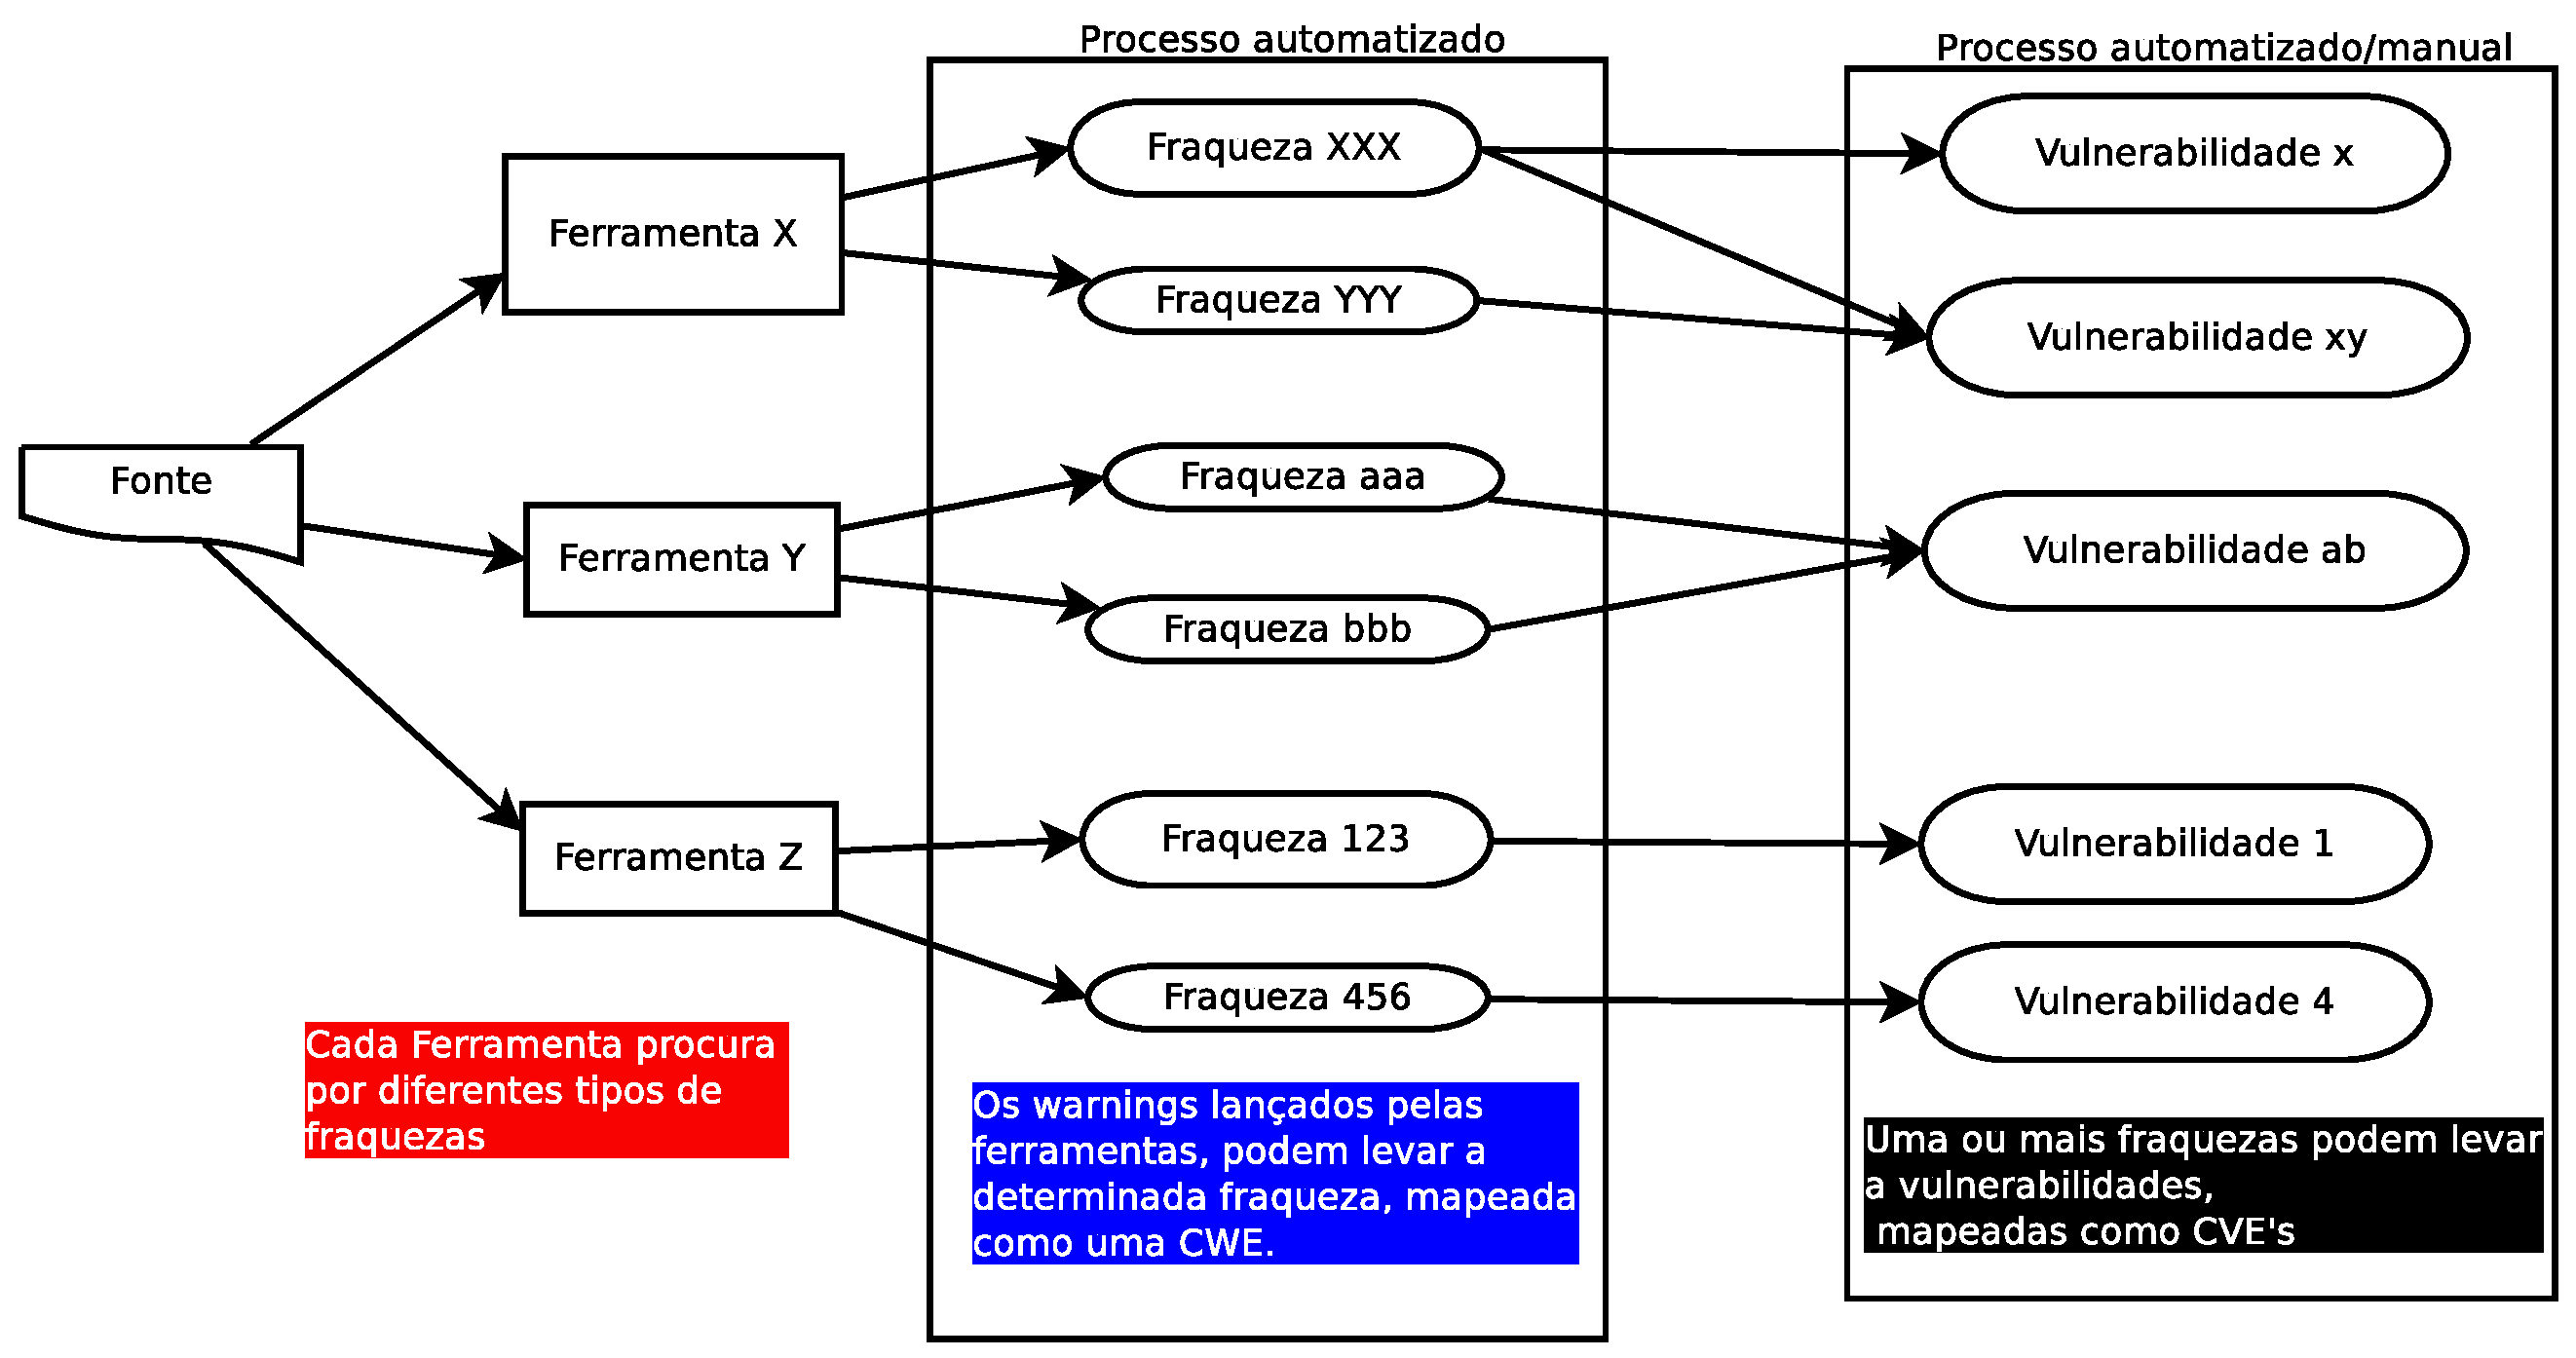
\includegraphics[scale=0.38]{figuras/vul1.eps}
%               \caption{Levantamento de vulnerabilidades}
%       \end{figure}

Além da $CWE$ existe um outro catálogo, chamado $CVE$. \
Este é responsável por, assim como a $CWE$, definir uma linguagem comum, \
mas para o registro de vulnerabilidades de segurança.

%\begin{figure}[h]
%        \centering
%        \label{fig03}
%        \includegraphics[scale=0.38]{figuras/lg_consensus.eps}
%        \caption{Visão Geral da CWE - retirado da pagina da CWE}
%\end{figure}

\section{Debian}
Segundo \cite{Zacchiroli}, pacotes são abstrações defininindo a \
granularidade em que usuários podem atuar(adicionar, \
remover, atualizar, etc) em um software disponível. \
Ainda segundo \cite{Zacchiroli} uma distribuição é uma coleção de \
pacotes mantidos de maneira coerente.  O Debian GNU/Linux, é uma \
distribuição do sistema operacional Linux, e os vários pacotes \
que são executados sobre ele\cite{Debian}.
O Linux é um clone do sistema operacional Unix, \
escrito do zero por por Linus Torvalds com a ajuda de um time de \
programadores distribuidos pelo internet \cite{Linux}.

O Debian Gnu/Linux é:
        \begin{itemize}
        \item \textbf{funcional}: Debian inclui 49.096 pacotes no \
                presente momento. O usuário pode escolher qual pacote \
                instalar;O Debian provê uma ferramenta
                para esse proposito.\cite{Debian}

        \item \textbf{livre para ser usado e redistribuido}: Não há um \
                consórcio ou pagamento exigido para participar na sua \
                distribuição e desenvolvimento.  Todos os pacotes que \
                são parte do Debian GNU/Linux são de distribuição livre, \
                usualmente sob os termos especificados
                pela licença GPL.\cite{Debian}

        \item \textbf{dinamico}: Com cerca de 1033 voluntários \
                contribuindo constantemente com código novo e melhorado,
                Debian evolui rapidamente.\cite{Debian}
        \end{itemize}


%TODO: Rever esse trexo e tirar o que nao for mais util
A estrutura de um pacote Debian é formalmente estabelecida por um documento \
chamado \textit {Debian Policy Manual}. Abordaremos esse documento de \
maneira mais profunda ao longo deste trabalho.Além de estabelecer a \
política que rege a distribuição como um todo,  esse manual também se \
atêm a definir a interface do sistema de gerenciamento de pacotes \
em que os desenvolvedores tem de estar familizarizados \cite{Guide}. \
É com \textit {Debian Policy Manual} que se define o que deve existir \
dentro de um pacote Debian. Além deste manual também estaremos \
utilizando como insumo para essa pesquisa o documento \
chamado \textit{Guide for Debian Maintainers}. Nesse guia prático, \
Osamu Aoki demonstra como um pacote Debian é construído, \
quais ferramentas são utilizadas, e como a política \
definida pelo \textit{Debian Policy Manual} deve ser implementada.
